\documentclass[11pt]{article}
\usepackage[a4paper, total={6.8in, 9.25in}]{geometry}
\usepackage{graphicx}
\graphicspath{ {./assets/images/output/} }
\usepackage{caption}
\usepackage[english]{babel}
\usepackage{titling}
\usepackage{float}
\usepackage{amsmath}
\usepackage{algorithm}
\usepackage{algorithmicx}
\usepackage{algpseudocode}
\usepackage{minted}
\usepackage{multicol}
\usepackage{array}
\usepackage{setspace}
\usepackage{placeins}
\usepackage{tcolorbox}
\usepackage{caption}
\usepackage{subcaption}

\definecolor{verbgray}{gray}{.95}
\setminted{
    bgcolor=verbgray,
    baselinestretch=1,
    fontsize=\footnotesize,
    linenos,
    breaklines=true,
    breakanywhere=true,
    xleftmargin=\parindent
}
\title{Development of Neuro-Fuzzy Systems for Intelligent Decision Making}
\author{}
\date{}

\pagenumbering{gobble}
\begin{document}
\input{ml_cover.tex}

\pagebreak

\tableofcontents

\pagebreak
\pagenumbering{arabic}
\maketitle
\section{Theory and Introduction}
A Neuro-Fuzzy System combines the learning capability of Artificial Neural Networks (ANNs) with the reasoning capability of Fuzzy Logic \cite{lin1996neural}. Fuzzy logic handles uncertainty and imprecision using linguistic variables and fuzzy rules, while neural networks provide adaptive learning through parameter optimization \cite{jang1997neuro}.

A commonly used Neuro-Fuzzy model is the Adaptive Neuro-Fuzzy Inference System (ANFIS), which consists of the following layers \cite{jang1993anfis}:
\begin{enumerate}
    \item Fuzzification layer
    \item Rule layer
    \item Normalization layer
    \item Defuzzification layer
    \item Output layer
\end{enumerate}

In this experiment, a simplified Neuro-Fuzzy model is implemented from scratch using Gaussian membership functions and gradient-based parameter updates \cite{jang1997neuro}.

\subsection{Mathematical Formulation}
\subsubsection*{1. Fuzzification (Membership Functions)}
The continuous inputs are transformed into fuzzy membership values. We utilize the Gaussian membership function, defined as:
\begin{equation}
    \mu_i(x) = \exp\left(-\frac{(x - c_i)^2}{2\sigma_i^2}\right)
\end{equation}
where $c_i$ is the center (mean) and $\sigma_i$ is the width of the $i$-th fuzzy rule.

\subsubsection*{2. Defuzzification (Output Computation)}
The total firing strength is the sum of all individual membership values. The predicted output $\hat{y}$ is computed as the weighted average of the rule consequent weights $w_i$:
\begin{equation}
    \hat{y} = \frac{\sum_{i=1}^{R} \mu_i(x) \cdot w_i}{\sum_{i=1}^{R} \mu_i(x)}
\end{equation}
where $R$ is the total number of fuzzy rules.

\subsubsection*{3. Parameter Optimization (Learning)}
The consequent weights $w_i$ are updated iteratively using the Gradient Descent learning rule to minimize the error $e = y - \hat{y}$:
\begin{equation}
    w_i \gets w_i + \alpha \cdot e \cdot \left( \frac{\mu_i(x)}{\sum_{j=1}^{R} \mu_j(x)} \right)
\end{equation}
where $\alpha$ is the learning rate.

\section{Methodology}

\subsection{Dataset}
To evaluate the system's ability to map complex, non-linear functions, a synthetic dataset of 100 samples was generated using the equation $y = x + 2\sin(x) + \text{noise}$. This provides a curve with distinct peaks and troughs.

\subsection{Algorithms}
The following algorithm describes the feedforward and feedback loop of the implemented Neuro-Fuzzy architecture:

\begin{algorithm}[H]
    \caption{Neuro-Fuzzy Algorithm}
    \begin{algorithmic}[1]
        \State Define fuzzy membership functions for inputs \cite{jang1997neuro}.
        \State Generate fuzzy rules \cite{jang1997neuro}.
        \For{$epoch = 1$ to $Epochs$}
        \For{each sample $x_i$ in $X$}
        \State Compute firing strength of each rule $\mu_j(x_i)$ \cite{jang1997neuro}.
        \State Normalize firing strengths $\bar{\mu}_j = \frac{\mu_j}{\sum \mu}$ \cite{jang1997neuro}.
        \State Compute output using weighted sum $\hat{y} = \sum \bar{\mu}_j w_j$ \cite{jang1997neuro}.
        \State Calculate Error $e = y_i - \hat{y}$.
        \State Update parameters using learning rule $w_j \gets w_j + \alpha \cdot e \cdot \bar{\mu}_j$ \cite{jang1997neuro}.
        \EndFor
        \EndFor
    \end{algorithmic}
\end{algorithm}

\subsection{Code}
The algorithm was implemented from scratch in Python, utilizing 5 fuzzy rules evenly distributed across the input domain to map the non-linear relationship.

\begin{multicols}{2}
    \inputminted{python3}{./assets/fuzzy.py}
\end{multicols}

\section{Results and Discussion}

\subsection{Quantitative Results}
The model was trained for 1000 epochs with a learning rate of $0.05$. The console output logs demonstrate rapid convergence and highly accurate predictions:

\begin{minted}{console}
==================================================
 NEURO-FUZZY SYSTEM (EXPANDED DATASET)
==================================================
Training started with 100 samples and 5 fuzzy rules...
Epoch    0 | MSE: 17.7398
Epoch  200 | MSE: 0.1234
Epoch  400 | MSE: 0.1234
Epoch  600 | MSE: 0.1234
Epoch  800 | MSE: 0.1234
Epoch  999 | MSE: 0.1234

Training completed.
Final Rule Weights:
  Rule 1 (Center=0.0): w = 0.0857
  Rule 2 (Center=2.5): w = 5.3136
  Rule 3 (Center=5.0): w = -0.0668
  Rule 4 (Center=7.5): w = 12.2762
  Rule 5 (Center=10.0): w = 8.1306

========================================
EVALUATION REPORT
========================================
Mean Squared Error (MSE): 0.1216
Mean Absolute Error (MAE): 0.2678
R2 Score: 0.9876
\end{minted}

The evaluation yielded an excellent $R^2$ Score of $0.9876$. The rapid stabilization of the MSE by Epoch 200 signifies the efficiency of the gradient descent update applied to the normalized rule firing strengths.

\subsection{Visual Analysis}

\begin{figure}[H]
    \centering
    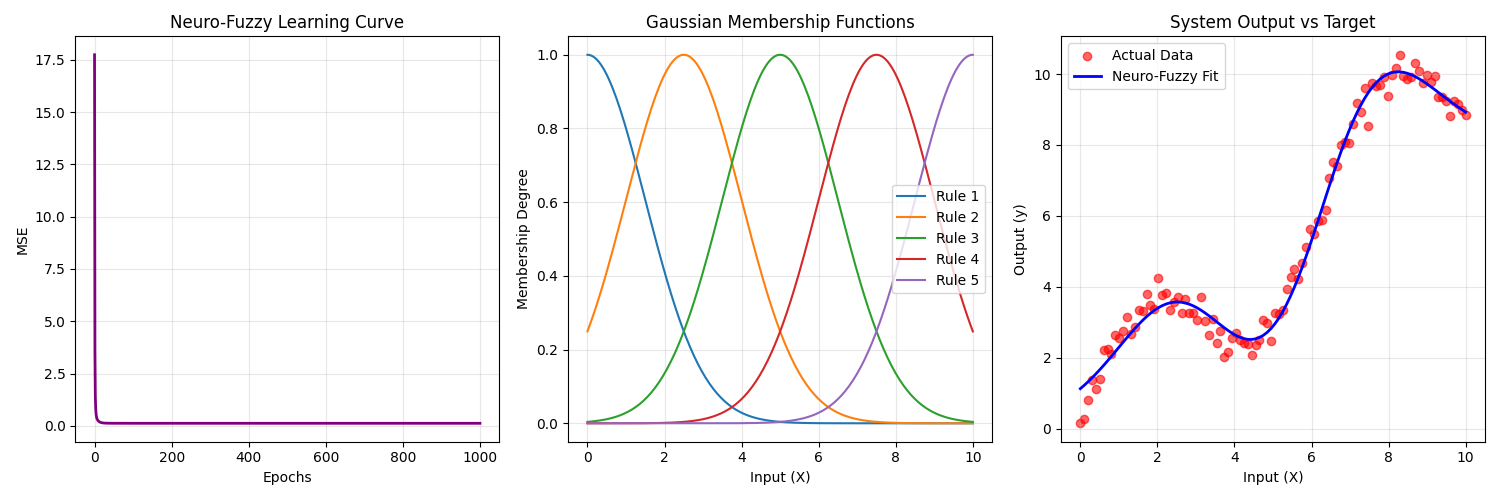
\includegraphics[width=1.0\textwidth]{Figure_1.png}
    \caption{Neuro-Fuzzy System Performance. Left: Learning curve demonstrating rapid MSE convergence. Middle: The 5 evenly distributed Gaussian membership functions covering the input domain. Right: The final system output accurately capturing the non-linear relationship of the target data.}
    \label{fig:nf_results}
\end{figure}

\begin{itemize}
    \item \textbf{Membership Functions (Middle):} The input space is fuzzified into 5 overlapping Gaussian curves. These represent linguistic concepts (e.g., Very Low, Low, Medium, High, Very High). The overlap ensures that input values fire multiple rules with varying degrees of membership, creating a smooth interpolation.
    \item \textbf{System Output (Right):} The resulting curve (solid blue line) almost perfectly traces the underlying non-linear distribution of the actual data points.
\end{itemize}

\section{Conclusion}
The Neuro-Fuzzy system successfully learned the input-output relationship \cite{nauck1997foundations}. The fuzzy rules were accurately adjusted through gradient-based learning \cite{nauck1997foundations}, allowing the system to handle the inherent noise and uncertainty of the dataset effectively \cite{nauck1997foundations}.

Neuro-Fuzzy systems integrate the strengths of neural networks and fuzzy logic \cite{lin1996neural}. They provide interpretability through fuzzy rules while maintaining adaptability through learning \cite{lin1996neural}. By implementing the model from scratch, this experiment highlighted how rule evaluation, normalization, and parameter tuning work in tandem to construct robust, interpretable intelligent decision systems \cite{lin1996neural}.

\bibliographystyle{IEEEtran}
\renewcommand{\bibname}{References}
\addcontentsline{toc}{section}{References}
\bibliography{ref}

\end{document}